\documentclass[aspectratio=169,t,xcolor=table]{beamer}
\usepackage[utf8]{inputenc}

\usepackage{booktabs} 
\usepackage{subcaption}

\usetheme{Ufg}
% remove caption Fig 
\usepackage{caption}
\captionsetup{labelformat=empty,labelsep=none}


\usepackage{pgfpages}
\setbeameroption{show notes}
\setbeameroption{show notes on second screen}

% link to video player
\usepackage{multimedia}

%tikz figures
\usepackage{tikzit}
\input{figs/dodstyle.tikzstyles}
%-------------------------------------theorems--------------
\newtheorem{conj}{Conjetura}
\newtheorem{defi}{Definição}
\newtheorem{teo}{Teorema}
\newtheorem{lema}{Lema}
\newtheorem{prop}{Proposição}
\newtheorem{cor}{Corolário}
\newtheorem{ex}{Exemplo}
\newtheorem{exer}{Exercício}

\setbeamertemplate{theorems}[numbered]
\setbeamertemplate{caption}[numbered]

%-------------------------------------------------------------%
%----------------------- Primary Definitions -----------------%

% This command set the default Color, is also possible to choose a custom color
\setPrimaryColor{orange} 

% First one is logo in title slide (we recommend use a horizontal image), and second one is the logo used in the remaining slides (we recommend use a square image)
    \setLogos{lib/logos/matfyz.png}{lib/logos/matfyz.png} 


% -------------------------------------- Title Slide Information
\begin{document}
\title[Inf UFG]{Multiagentní hledání cest (s protivníkem)}
%\subtitle{Template Latex}

\author{Marika Ivanová}

\institute[UFG] % (optional)
{
  \inst~
  Katedra teoretické informatiky a matematické logiky (KTIML)\\
  ~\newline
  MFF UK
  ~\newline
  ~\newline
  ivanova@ktiml.mff.cuni.cz

}
%-----------------------The next statement creates the title page.
\frame[noframenumbering]{
	\titlepage

	\note{
		Dobrý den, vítejte na virtuálním dni otevřených dveří na matfyzu. 
		V tomto videu budeme diskutovat téma Multiagentního hledání cest s protivníkem, což je jedna z oblastí umělé inteligence.
		Nejdříve si povíme něco o Multiagentního hledání cest a poté ukážeme, jak se tento problém rozšíří o element protivníka.
	}

}


%------------------------------------------------Slide 1
%\setLayout{vertical} % This command define the layout. 'vertical' can be replace with 'horizontal', 'blank, 'mainpoint', 'titlepage'
%
%\begin{frame}
%    \frametitle{Table of Contents}
%    \tableofcontents
%\end{frame}
%---------------------------------------------------------


%---------------------------------------------------------Slide 2
\section{Multiagentní hledání cest}

\setLayout{horizontal}
\begin{frame}
    \frametitle{Multiagentní hledání cest}
    \textbf{Popis problému}
    \begin{itemize}
        \item Skupina agentů (robotů) rozmístěných v daném prostředí
        \item Každý agent má definovanou počáteční a cílovou pozici
        \item \textbf{Úkol:} Přemístit agenty na cílové pozice aniž by došlo ke kolizi 
    \end{itemize}
    ~\newline
    \textbf{Účelová funkce:}
    \begin{itemize}
        \item Minimalizovat čas dojetí posledního agenta (makespan)
        \item Minimalizovat součet počtu přesunů agentů (total distance)
        \item Minimalizovat součet časů jednotlivých agentů (total arrival time)
    \end{itemize}

	\note{
		Uvažujme skupinu agentů, například robotů rozmístěných v nějakém prostředí s překážkami.
		Každý agent má zadefinovánu počáteční a cílovou pozici.
		Naším úkolem je navigovat agenty do jejich jednotlivých cílových pozic, aniž by do sebe nebo do překážek po cestě naráželi.

		Nejen že se snažíme dosáhnout cílových pozic, ale rádi bychom to udělali co nejlépe.
		Existuje několik kritérií pro posouzení kvality řešení.
		Nejtypičtěji se používá takzvaný minimum makespan, neboli snažíme se o co nejkratší čas dojetí posledního agenta do svého cíle.
		Dále je možnost minimalizovat počet přesunů, tedy snažíme se, aby agenti celkově urazili co nejmenší vzdálenost.
		Nebo lze také minimalizovat celkový čas, který agenti stráví na cestě.
	}
	
\end{frame}

%---------------------------------------------------------Slide 3
\setLayout{vertical}
\begin{frame}
\frametitle{Motivace}
\begin{columns}
\begin{column}{.5\textwidth}
\begin{itemize}
    \item Přemísťování zboží ve skladech
    \item Manipulace s lodními kontejnery
    \item Navigování skupiny autonomních vozidel
\end{itemize}
\begin{figure}
        \centering
        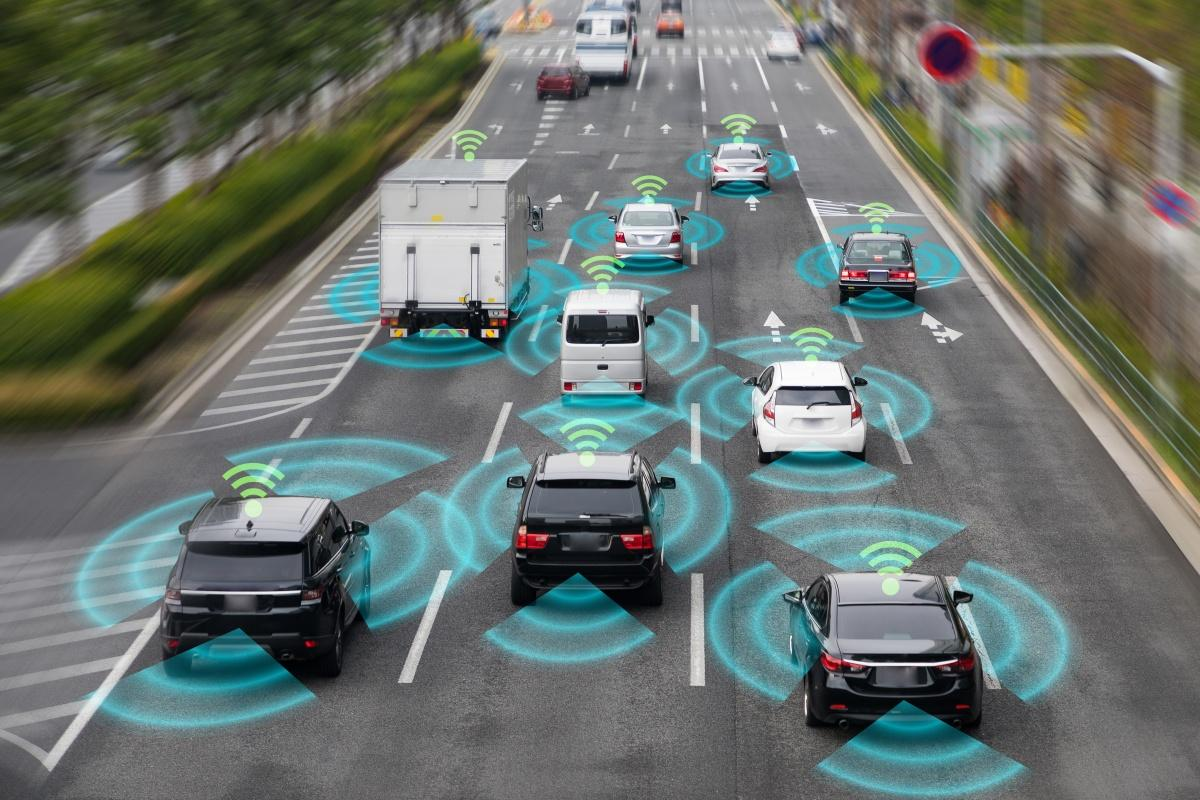
\includegraphics[width=.7\textwidth]{figs/autonomous-car.jpg}
    \end{figure}
 
\end{column}
\begin{column}{.4\textwidth}
    \begin{figure}
        \centering
        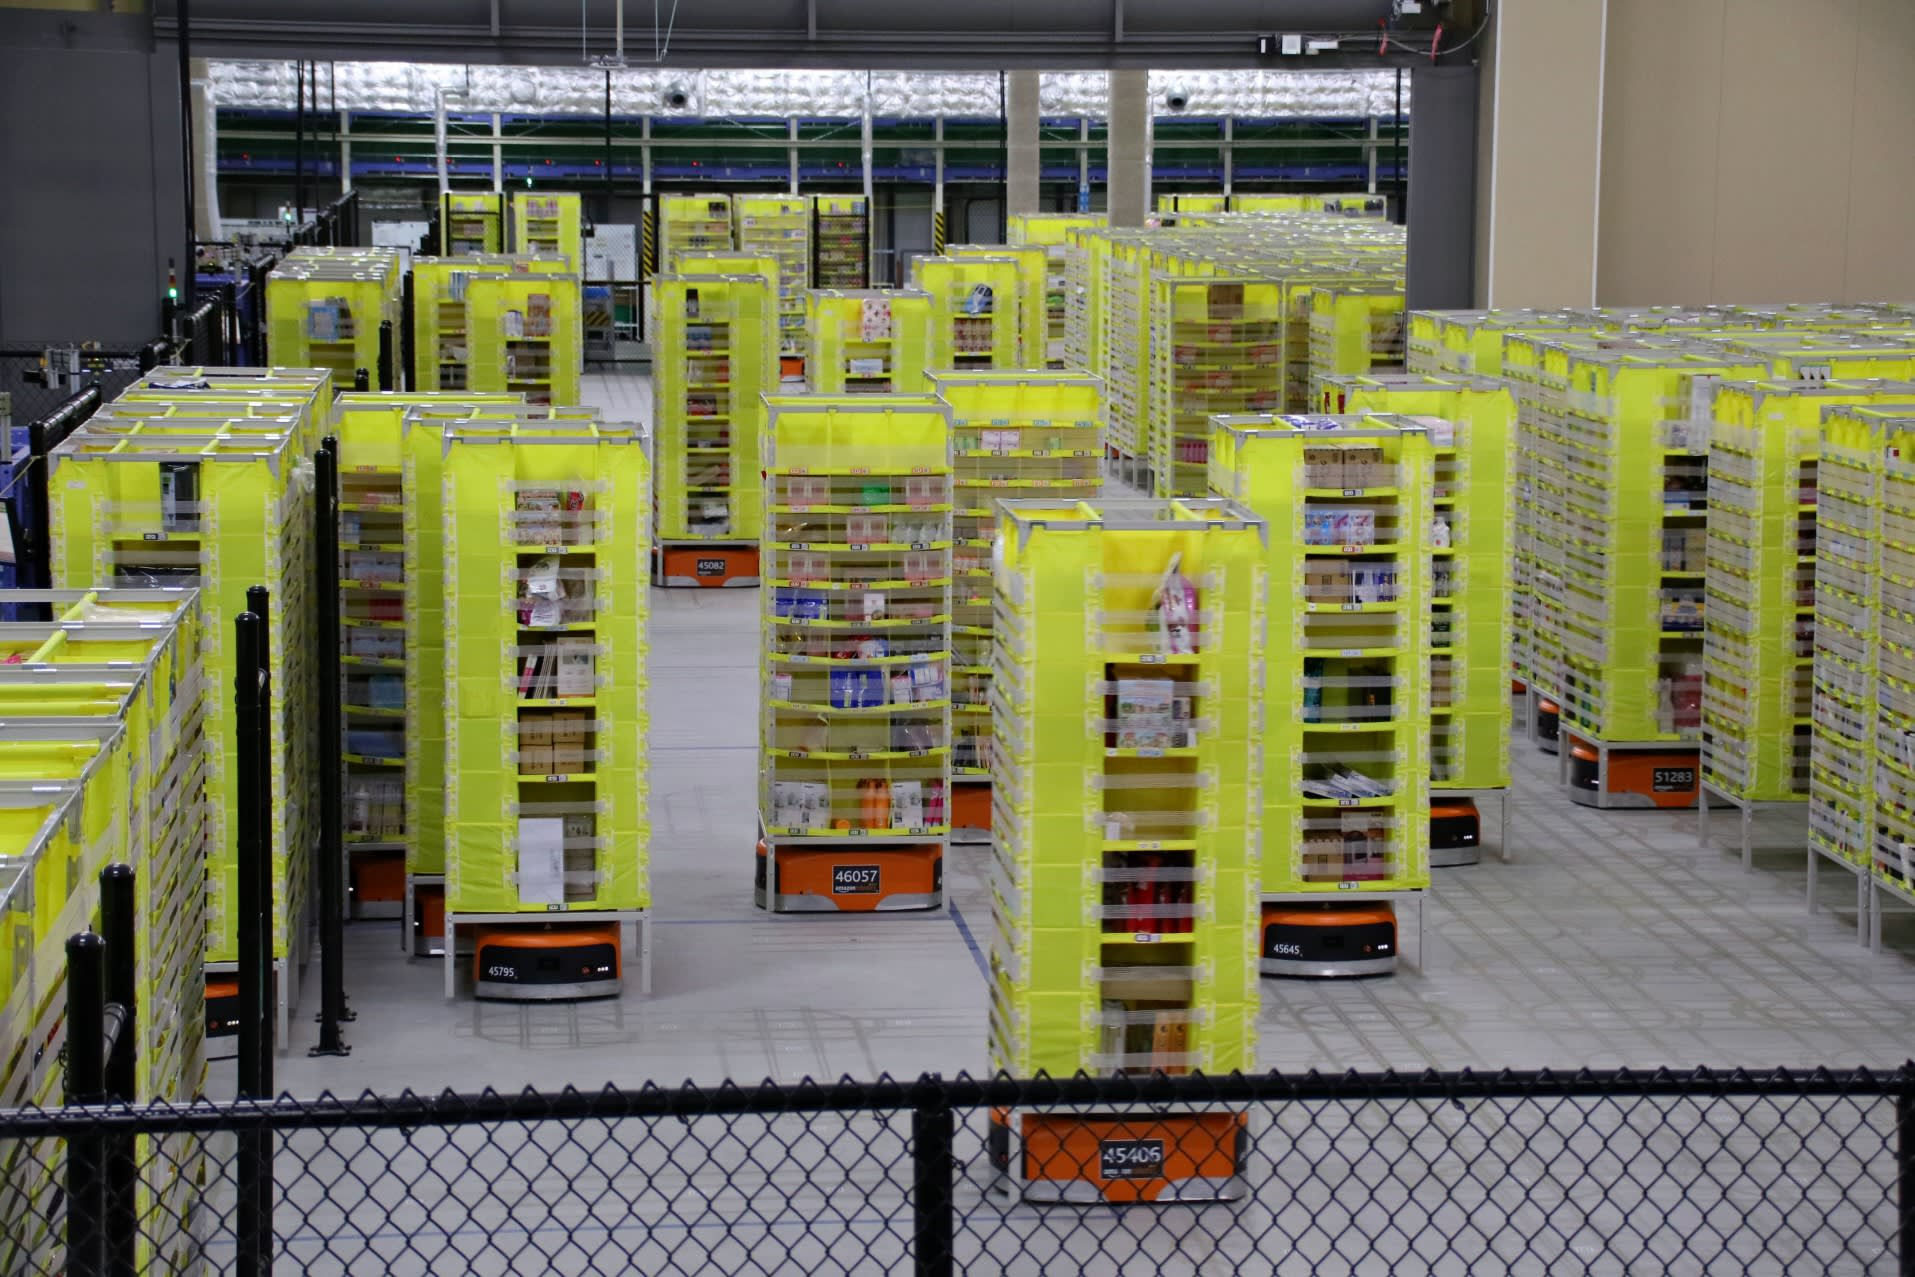
\includegraphics[width=.7\textwidth]{figs/roboti-amazon.jpg}
    \end{figure}
    
     \begin{figure}
        \centering
        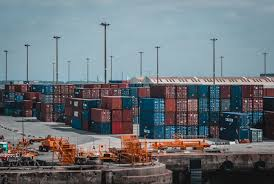
\includegraphics[width=.7\textwidth]{figs/shipping.jpg}
    \end{figure}
\end{column}
\begin{column}{.1\textwidth}
~
\end{column}
\end{columns}
	\note{
		Tento problém je motivován řadou praktických aplikací.
		V poslední době se ve velkých skladech nasazují roboti, kteří musejí přemisťovat zboží či celé regály z místa na místo.
		Další aplikací v logistice je přemísťování lodních kontejnerů. 
		Agenti jsou v tomto případě kontejnery. 
		Je zřejmé, že přemísťování takových velkých objektů je vhodné provést co nejefektivněji.
		Dalším poměrně žhavým tématem je ovládání autonomních vozidel, zejména v dopravních špičkách.
	}

\end{frame}
\begin{frame}

\centering
\href{run:/usr/bin/xdg-open -fs vid/amazon.mp4}{
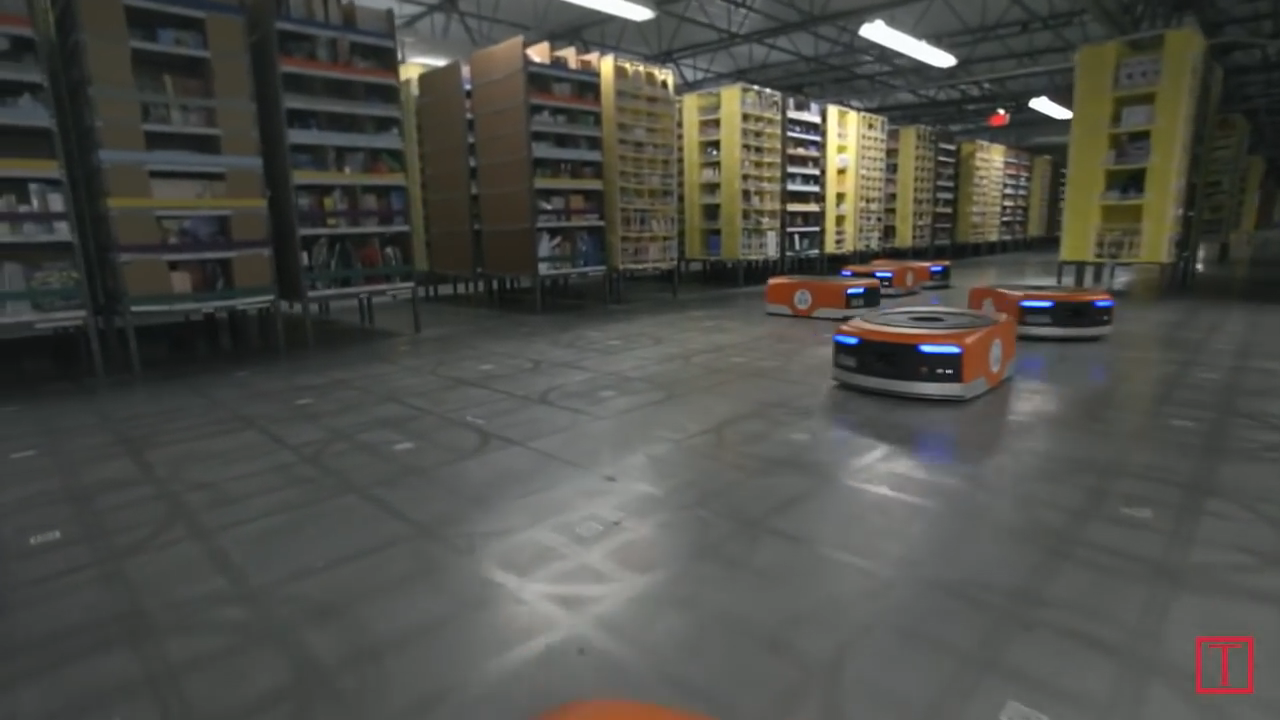
\includegraphics[scale=0.25]
{figs/amazon.png}}
\note{
	Zde je krátká video ukazující jak se kiwa roboti pohybují ve skladu v amazonu.
	Vidíme zde skupinu robotů, kteří se potřebují dopravit na určité místo a nesmí kolidovat.
	}
\end{frame}
%---------------------------------------------------------Slide 3
\begin{frame}
\frametitle{Abstrakce problému}
\begin{columns}
\begin{column}{.4\textwidth}
    \begin{figure}
        \vspace{-20pt}
        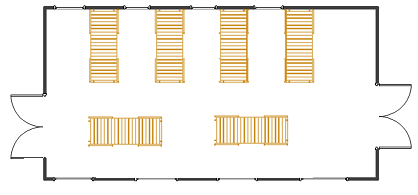
\includegraphics[width=1\textwidth]{figs/warehouse-plan-transp.png}
        %\caption{Template's Layouts.}
        %\label{fig:layouts}
    \end{figure}
    
     \begin{figure}
        \hspace{-10pt}
        \vspace{-30pt}
        \tikzfig{figs/warehouse-graph}
        %\caption{Template's Layouts.}
        %\label{fig:layouts}
    \end{figure}
\end{column}
\begin{column}{.6\textwidth}
\begin{itemize}
\item Matematická formulace nezbytná pro teoretické studium i počítačové zpracování
\item Prostředí modelujeme pomocí grafu
    \begin{itemize}
    \item Graf - množina vrcholů a hran
    \item vrcholy - možná umístění agentů
    \item hrany spojují sousední umístění 
    \end{itemize}
    \item Definice počátečních a cílových pozic
\end{itemize}

\end{column}

\end{columns}
	\note{
		Abychom mohli problém studovat ať už teoreticky, či provádět simulace, je nezbytné jej formálně zadefinovat.
		Prostředí, ve kterém jsou agenti rozmístěni modelujeme pomocí grafu.
		Graf je matematická struktura sestávající z množiny vrcholů a hran.
		Vrcholy jsou body a hrany jsou spojnice mezi nimi.
		Vrcholy reprezentují možná umístění agentů, hrany pak spojují přilehlá umístění
		Zde na horním obrázku vidíme příklad plánu nějakého skladu.
		Pro každou pozici, na které může robot stát máme vrchol.
		Předpokládáme, že se roboti můžou pohybovat ve čtyřech směrech, a tedy nám vzniknem mřížkový graf jako na spodním obrázku.
	}
	
\end{frame}
%---------------------------------------------------------Slide 4
\begin{frame}
\frametitle{Pravidla pohybu}
\begin{itemize}
    \item Každý agent umístěn v jednom vrcholu
    \item Čas rozdělen na diskrétní kroky
    \item V každém kroku se agent pohybuje podél hrany nebo stojí na místě
    \item Agent se může posunout do vrcholu opouštěného jiným agentem ve stejném kroku
    \item 2 agenti si nesmí vyměnit pozice v jednom kroku
\end{itemize}
\begin{columns}
    \begin{column}{.5\textwidth}
    \begin{figure}
        \centering
        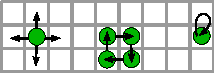
\includegraphics[width=.7\textwidth]{figs/moves.pdf}
        \end{figure}
    \end{column} 
    \begin{column}{.5\textwidth}
        \begin{figure}
        \centering
        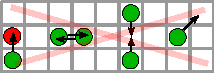
\includegraphics[width=.7\textwidth]{figs/nomovesx.pdf}
    \end{figure}
    \end{column}
\end{columns}
	\note{
		Dále je třeba zadefinovat pravidla, podle kterých se agenti pohybují.
		Každý agent je umístěn v právě jednom vrcholu.
		Spojitý čas rozdělujeme na diskrétní kroky, například vteřiny.
		V jednom časovém kroku se agent může přesunout na sousední vrchol podél hrany, nebo také může zůstat stát na místě.
		Rovněž je povolen přesun agenta na vrchol, který je současně opouštěn jiným agentem- jako vagony vlaku.
		Výjimkou k tomuto pravidlu je případ, kdy by si 2 agenti pouze vyměnili pozice - to povoleno není.
		
	}
\end{frame}
%---------------------------------------------------------Slide 5
\setLayout{horizontal}
\begin{frame}
\frametitle{Multiagentní hledání cest}
\begin{columns}
\begin{column}{.5\textwidth}
    \begin{figure}
    \begin{overprint} 
        \onslide<1>\tikzfig{figs/mapfex-makespan-1}
        \onslide<2>\tikzfig{figs/mapfex-makespan-2}
        \onslide<3>\tikzfig{figs/mapfex-makespan-3}
        \onslide<4->\tikzfig{figs/mapfex-makespan-4}
    \end{overprint} 
    \end{figure}
    
\end{column}
\begin{column}{.5\textwidth}
    \begin{figure}
    \begin{overprint} 
        \onslide<5>\tikzfig{figs/mapfex-sum-1}
        \onslide<6>\tikzfig{figs/mapfex-sum-2}
        \onslide<7>\tikzfig{figs/mapfex-sum-3}
        \onslide<8>\tikzfig{figs/mapfex-sum-4}
        \onslide<9>\tikzfig{figs/mapfex-sum-5}
    \end{overprint} 
    \end{figure}
    
\end{column}
\end{columns}
\begin{columns}
\begin{column}{.5\textwidth}
    \only<1>{
    \begin{itemize}
     \item[] makespan: \textcolor{red}{0} 
     \item[] sum-of-costs: 0
    \end{itemize}
     }
    \only<2>{
        \begin{itemize}
        \item[] makespan: \textcolor{red}{1}
        \item[] sum-of-costs: 2
        \end{itemize}
    }
    \only<3>{
        \begin{itemize}
    \item[] makespan: \textcolor{red}{2}    
    \item[] sum-of-costs: 4
        \end{itemize}
    }
    \only<4->{
        \begin{itemize}
    \item[] makespan: \textcolor{red}{3} 
    \item[] sum-of-costs: 6
        \end{itemize}
    }
\end{column}
\begin{column}{.5\textwidth}
    \only<5>{
        \begin{itemize}
    \item[] makespan: \textcolor{red}{0} 
    \item[] sum-of-costs: 0
        \end{itemize}
    }
    \only<6>{
        \begin{itemize}
    \item[] makespan: \textcolor{red}{1} 
    \item[] sum-of-costs: 2
        \end{itemize}
    }
    \only<7>{
        \begin{itemize}
    \item[] makespan: \textcolor{red}{2}    
    \item[] sum-of-costs: 3
        \end{itemize}
    }
    \only<8>{
        \begin{itemize}
    \item[] makespan: \textcolor{red}{3} 
    \item[] sum-of-costs: 4
        \end{itemize}
    }
    \only<9->{
        \begin{itemize}
    \item[] makespan: \textcolor{red}{4} 
    \item[] sum-of-costs: 5
        \end{itemize}
    }
\end{column}
\end{columns}
	\note{	
		Nyní si ukážeme příklad velmi jednoduché instance se dvěma agenty. 
		Zakroužkované vrcholy představují císle agentů.
		Podíváme se, jaké je optimální řešení pro nejmenší makespan, tedy nejkratší čas dojetí posledního agenta.
		Ačkoli a2 stojí hned vedle svého cíle, v prvním kroku se do n2j neposune.
		Misto toho A1 specha po nejkratší cestě ke svému cíli.
		A2 tedy jakoby dává přednost agentovi a1. 
		Když A1 provádí poslední krok, může se i A2 přemístit do svého cíle. 
		Toto řešení má makespan 3, zatímco celkový čas jednotlivých agentů je 6.

		Nyní uvidíme řešení, které má sice horší makespan, ale lepší součet časů jednotlivých agentů.
		V tomto řešení A2 okamžitě dorazí do cíle, zatímco A1 jej musí objet po delší cestě. 
		Toto řešení má součet časů 5, což je optimální.
		Naopak makespan je 4, což lze udělat lépe, jak jsme viděli na předchozím případě.
	}
\end{frame}
%---------------------------------------------------------Slide 5
\begin{frame}
\frametitle{Řešící metody}
\begin{enumerate}
    \item<1-> Centralizované 
        \begin{itemize}
        \item<2-> Agenti považováni za jednu entitu
        \item<2-> Cesty se hledají simultánně
        \end{itemize}
        \vspace{20pt}
    \item<1-> Decentralizované
        \begin{itemize}
        \item<3-> Agenti zpracováváni jednotlivě
        \end{itemize}
	\item[]<4-> Centralizované metody dávají typicky lepší řešení, ale jsou výpočetně náročnější
\end{enumerate}
	\note{	
		Řešící metody lze rozdělit na 2 základní skupiny - Centralizované a decentralizované.
		U centralizovaných metod je celá skupina agentů považována za jednu entitu.
		Cesty jsou tedy hledány současně pro všechny agenty.
		U decentralizovaných metod jsou cesty pro agenty hledány postupně.
		Výsledné řešení u centralizovaných metod bývá typicky lepší než u decentralizovaných metod, ovšem centralizované metody bývají často výpočetně náročnější.
	}

\end{frame}

%---------------------------------------------------------Slide 6
\setLayout{vertical}
\begin{frame}
\frametitle{Multiagentní hledání cest  \\\textcolor{orange}{s protivníkem} (AMAPF)}
\begin{columns}
\begin{column}{.65\textwidth}
\begin{itemize}
    \item Zobecnění MAPF
    \item Agenti rozděleni do dvou soupeřících týmů
    \begin{itemize}
        \item<2-> \textcolor{orange}{Útočníci $A$} 
        \item<2-> \textcolor{orange}{Obránci $D$} 
    \end{itemize}
        \item<3-> Útočníci se snaží dosáhnout cílových pozic
        \item<3-> Obránci v tom brání
    \item<4-> Hra dvou hráčů
    \item<4-> Týmy se střídají na tahu v každém kroku
    \item<5-> \textbf{Motivace: } vojenské a bezpečnostní simulace, herní průmysl
\end{itemize}
\end{column}
\begin{column}{.35\textwidth}
        \begin{figure}
        \hspace{-60pt}
        \vspace{-40pt}
        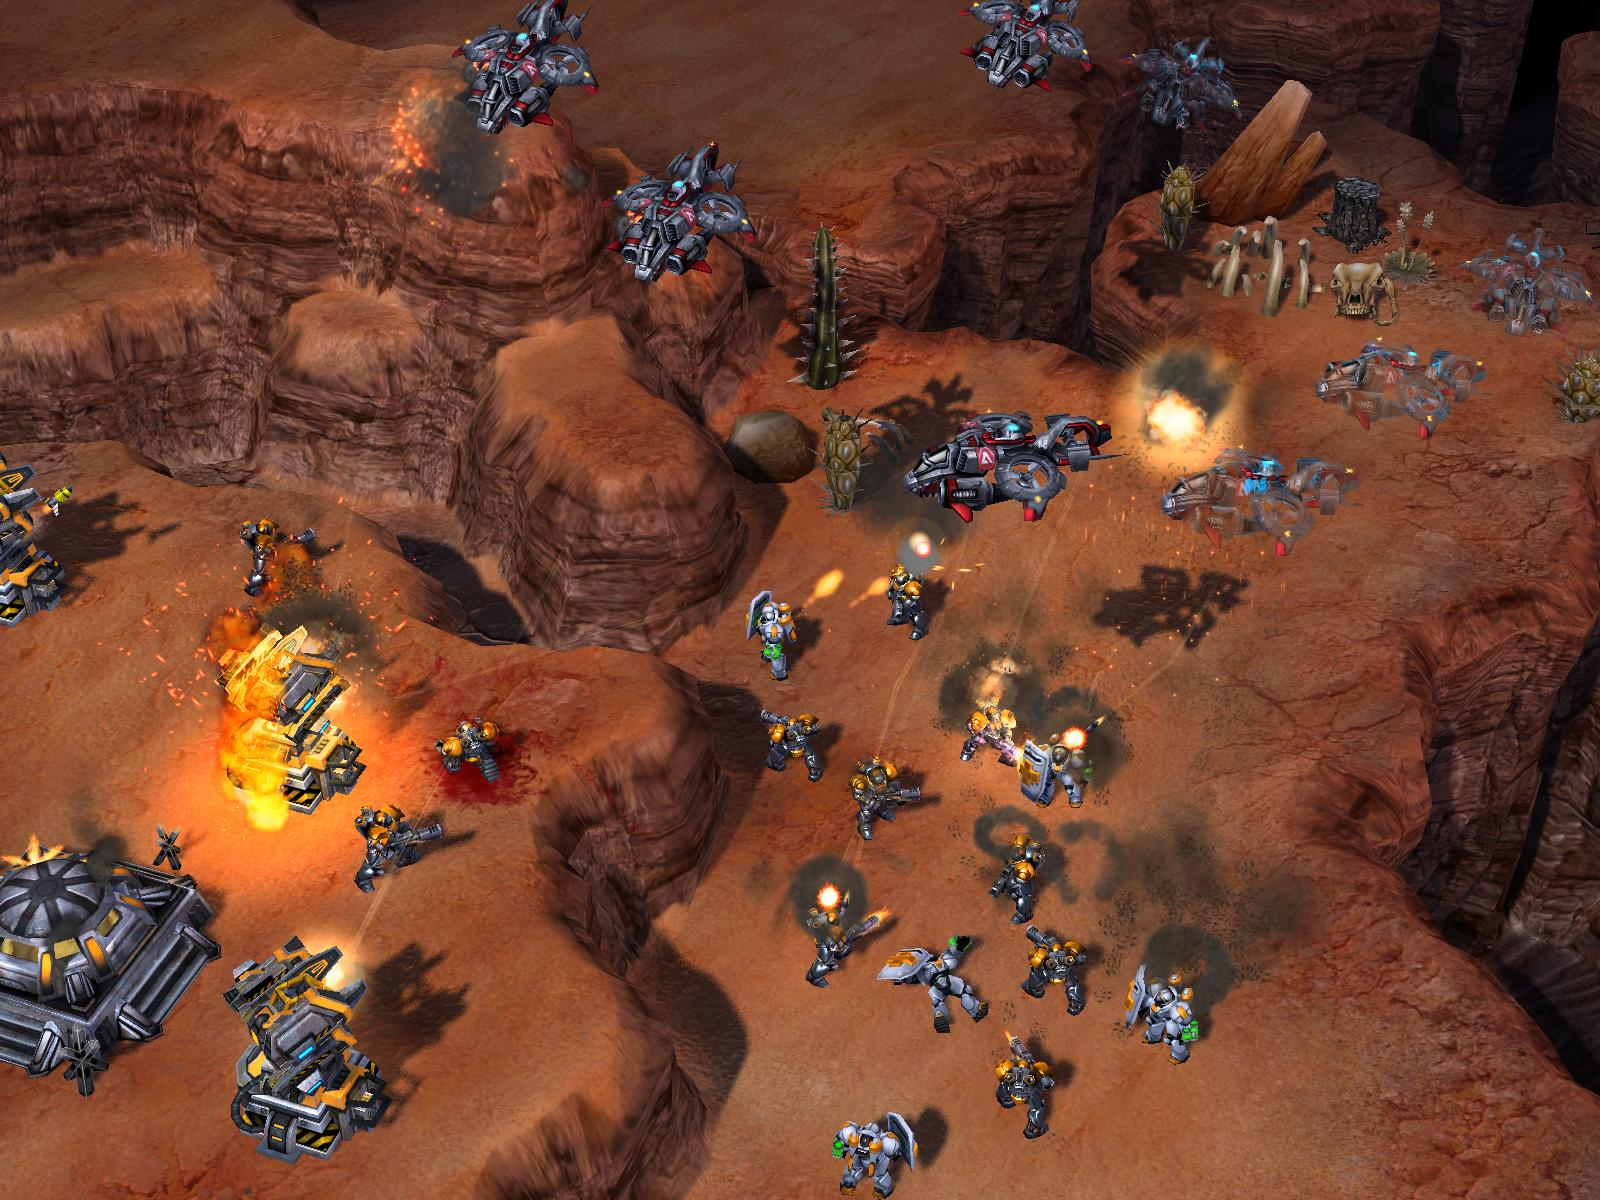
\includegraphics[width=.8\textwidth]{figs/game.jpg}
    \end{figure}
\end{column}
\end{columns}
	\note{	
		Zobecnění problému představuje zavedení elementu protivníka do multiagentního hledání cest.
		Agenti jsou rozděleni do dvou týmů nazývaných ÚTOČNÍCI a OBRÁNCI. 
		Úkolem útočníka je stejný jako jsme dosud viděli, tedy přemístit agenty na cílové pozice aniž by kolidovali.
		Obránci se naopak snaží uchránit tyto cíle před útočníky.
		Problém se tedy stává hrou dvou hráčů, kdy se jednotlivé týmy střídají na tahu.
	}
\end{frame}
%---------------------------------------------------------Slide 7
\begin{frame}
\frametitle{Multiagentní hledání cest  \\\textcolor{orange}{s protivníkem} (AMAPF)}
\begin{itemize}
    \item[]<1-> \textbf{Výhra útočníka:} Všichni agenti z týmu $A$ dosáhnou svých cílů
    \item[]<1-> \textbf{Problém:} nalézt vyhrávající strategii pro tým $A$
\end{itemize}
\begin{block}<2->
{Vyhrávající strategie}
V každém kroku, kdy je tým $A$ na tahu, zahrát takový tah, že $A$ vyhraje bez ohledu na odpověď soupeře $D$ 
\end{block}
\vspace{20pt}
\begin{itemize}
	\item<3-> Rozhodnutí, zda existuje vyhrávající strategie je velmi těžké\\ (\textcolor{orange}{PSPACE těžké})
	\item<4-> Zdá se ale, že je to ještě těžší (\textcolor{orange}{EXPTIME těžké})
\item<5-> Na MFF se dozvíte, co to znamená :)
\end{itemize}
	\note{	
		Výhra týmu útočníků nastane v případě, že se všem agentům podaří dojet na své cíle.
		Naším úkolem je nalézt vítěznou strategii pro útočníky.
		Vyhrávající strategie znamená, že v každém kroku, kdy jsou útočníci na tahu, zahrají takový tah, že obránci nemohou zabránit vítězství útočníka ať hrají jakkoli.
		Teoretické studium tohoto problému ukazuje, že už jen rozhodnutí, zda nějaká vyhrávající strategie pro útočníka existuje je velmi těžké, konkrétně PSPACE- těžké. 
		V poslední době se ale zdá, že je to ještě těžší, neboli EXPTIME těžké.
		Co tyto pojmy přesně znamenají si řekneme až na matfyzu.
	}

\end{frame}

\begin{frame}
	\frametitle{Ukázka pohybu agentů v AMAPF instanci}
	\note{
		Nyní se podíváme na krátkou vizualizaci pohybu agentů v AMAPF.
		Tři světle zelení agenti  4, 5, a 6 nahoře mají tři tmavě zelené cile dole.
		Agent č. 3 má cíl ve zbývajícím tmavě zeleném vrcholu vpravo nahoře.
		Podívejme se, jaké posuny musí agenti udělat, aby červení útočníci jim nezabránili v dosažení cílů.

	}
\end{frame}
%---------------------------------------------------------Slide 8
\setLayout{horizontal}
\begin{frame}
\frametitle{Řešící metody}
	\begin{itemize}
		\item V typické instanci se nepodaří všem útočníkům dojet do cíle
		\item Snažíme se tedy o obsazení co největšího počtu cílů
	\end{itemize}
\begin{columns}
	\vspace{20pt}
\begin{column}{.33\textwidth}
\textbf{Hladové}\newline

                Provede se tah jevící se v danou chvíli nejlépe. Posuzováno dle různých kritérií.
\end{column}
\begin{column}{.33\textwidth}
\textbf{Herní}\newline

                Klasické (alpha-beta) i méně známé algoritmy (Monte Carlo tree search)
                používané ve hrách dvou hráčů jako šachy nebo go.
\end{column}
\begin{column}{.33\textwidth}
\textbf{MAPF}\newline

                Rozšíření metod navržených pro MAPF o element protivníka.
\end{column}
\end{columns}
    	\note{	
		Ve velké většině případů se nepodaří úplně všem agentům útočníkům dojet do cíle.
		Snažíme se tedy o to, aby co největší počet útočníků dojel do cíle.
		Navrhujeme algoritmy, které dostanou na vstupu nějakou instanci problému a vždy když je útočník na tahu zvolí, jaký krok mají agenti provést.
		Zatím jsme zkoumali 3 různé typy algoritmů.
		Nejjednodušší hladové metody zahrají vždy takový tah, který vede do nejlepší pozice.
		To může být často hodně krátkozraké.
		Naopak herní algoritmy jako minimax, alpha beta a podobné se snaží dívat dál dopředu a zahrát takový tah, který vede k nelepšímu možnému výsledku za určitý časový úsek.
		pro Multiagentní hledání cest bez protivníka bylo navrženo mnoho řešících algoritmů. 
		Je tedy možné se z nich inspirovat a upravit je tak, aby v sobě měly element protivníka zahrnutý.
	}

\end{frame}
%--------------------------------------------------------- Slite 9
\begin{frame}
\frametitle{Budoucí výzkum}
\begin{itemize}
    \item[] MAPF je již mnoho let intenzivně studován
    \item[] Naopak AMAPF je spíše v začátcích
    \item[] 
    \item[] Možné směry dalšího výzkumu:
    
        \begin{itemize}
        \item Výpočetní složitost speciálních variant
        \item Podrobnější srovnání řešících algoritmů
        \item Návrh nových řešících technik
        \item Strategie pro tým obránců
	\item Studium modifikací problému (např. ne všichni agenti mají cíle)
        \end{itemize}
\end{itemize}
	\note{	
		Multiagentní hledání cest s protivníkem představuje téma s velmi dobrým výzkumným potenciálem.
		Lze jej studovat teoreticky i prakticky, a v obou směrech lze očekávat zajímavé výsledky, 
		které bude možno publikovat na mezinárodních konferencích o umělé inteligenci a příbuzných tématech.
		}
\end{frame}
\begin{frame}
	\frametitle{Zdroje}
	\begin{enumerate}
		\item Adversarial Cooperative Path-Finding: Complexity and Algorithms, 2014 IEEE 26th International Conference on Tools with Artificial Intelligence
		\item Adversarial Cooperative Path-Finding: A First View, AAAI (Late-Breaking Developments) 2013
		\item www.koupy.net/graphrec.php
		\item www.therobotreport.com
		\item www.smartcitiesworld.net
	\end{enumerate}
	\note{
		Tímto bych tedy ráda prezentaci zakončila. 
		Děkuji za shlédnutí a doufám, že již brzy bude situace příznivější a bude možné se sektat osobně.

	}

\end{frame}


\end{document}
